\chapter{Application}
\label{chap:application}
%#############################################################################################


%#############################################################################################
\section{Assignment 3: ROC Curve}
\label{assignment3}

In this assignment, the ROC curve of a simple 1D-toy data set with two classes should be plotted. Each class is normal with standard deviation one and identical priors. Figure~\ref{fig:roc_curve} depicts the ROC curve of the data set. Four sample sizes are used to generate the ROC curve: 10, 100, 1000 and 10000.

\begin{figure}[h!]
	\centering
	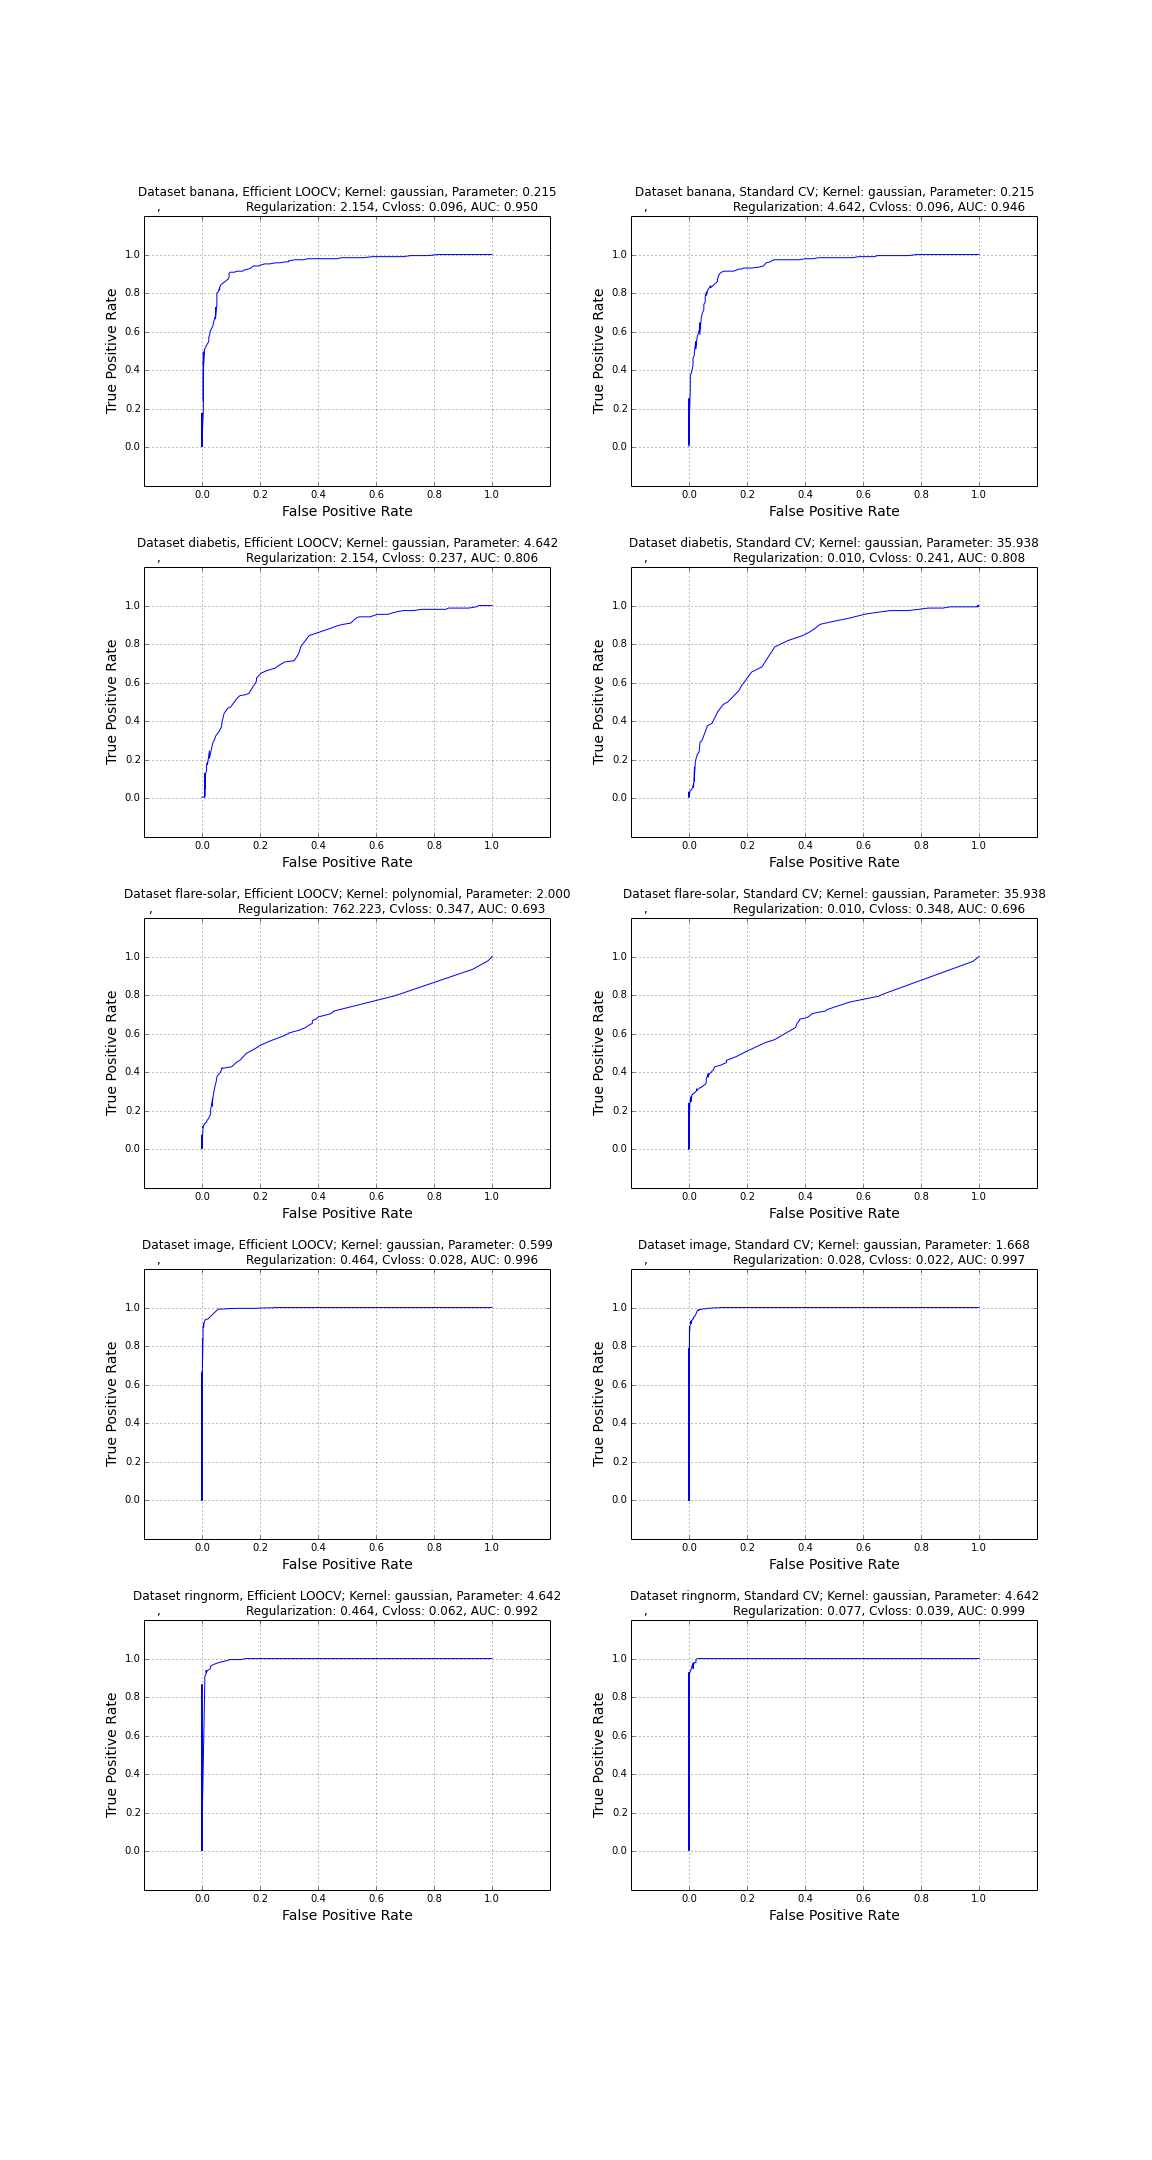
\includegraphics[scale=0.4983]{roc_curve}
	\caption{ROC curve with different sample sizes}
	\label{fig:roc_curve}
\end{figure}


%#############################################################################################
\section{Assignment 4: Kernel Ridge Regression}
\label{assignment4}

In this assignment, the \textit{krr} should be applied to five data sets: \textit{banana}, \textit{diabetis}, \textit{flare-solar}, \textit{image} and \textit{ringnorm}. \textit{krr} should be applied to each data set using efficient cross-validation and then finds the best classifier by cross-validation. The normal CV takes a longer time than the efficient LOOCV to optimize the regularization, because it has to cross-validate all of the folds and calculate the inverse matrix. On the other hand, the efficient LOOCV only do one inverse in order to get the optimal regularization parameter. Furthermore, the inverse of efficient LOOCV is only an inverse of a diagonal matrix which can be easily calculated by inverting the diagonal. Table~\ref{tab:cv} shows the optimal parameters for each data set.

From the experiment, it turned out that gaussian kernel is the optimal kernel for all data sets. But i think the regularization parameter obtained by the efficient LOOCV was wrong, because it is always 1.8 for all data sets. I think the reason for that is because the eigenvalues of the kernel matrix $K$ used for $c$ in efficient LOOCV are very small values, so that it always return $mean=1$. Unfortunately, i cannot find where the mistake is. The whole experiment took about 6 hours. The longest CV execution is by \textit{image} data set which took about 
3.5 hours.

\begin{table}
\begin{tabular}{l*{6}{c}r}
\centering
\textbf{Dataset}  & \textbf{Kernel} & \textbf{Kernelparameter} &  \textbf{Cvloss} & \textbf{Regularization} & \textbf{Time (in seconds)} \\
\hline
Banana & Gaussian & 0.215 & 0.099 & 1.80 & 272.435  \\
Diabetis            & Gaussian & 4.641 & 0.243 & 1.80 & 584.214  \\
Flare-Solar           & Gaussian & 4.641 & 0.354 & 1.80 & 949.138  \\
Image     & Gaussian & 0.599 & 0.029 & 1.80  & 12544.090 \\
Ringnorm     & Gaussian & 0.077 & 0.046 & 1.80 & 291.681 \\
\end{tabular}
\caption{The optimal parameters for each data set}
\label{tab:cv}
\end{table}




